% Options for packages loaded elsewhere
\PassOptionsToPackage{unicode}{hyperref}
\PassOptionsToPackage{hyphens}{url}
%
\documentclass[
]{report}
\usepackage{lmodern}
\usepackage{amssymb,amsmath}
\usepackage{ifxetex,ifluatex}
\ifnum 0\ifxetex 1\fi\ifluatex 1\fi=0 % if pdftex
  \usepackage[T1]{fontenc}
  \usepackage[utf8]{inputenc}
  \usepackage{textcomp} % provide euro and other symbols
\else % if luatex or xetex
  \usepackage{unicode-math}
  \defaultfontfeatures{Scale=MatchLowercase}
  \defaultfontfeatures[\rmfamily]{Ligatures=TeX,Scale=1}
\fi
% Use upquote if available, for straight quotes in verbatim environments
\IfFileExists{upquote.sty}{\usepackage{upquote}}{}
\IfFileExists{microtype.sty}{% use microtype if available
  \usepackage[]{microtype}
  \UseMicrotypeSet[protrusion]{basicmath} % disable protrusion for tt fonts
}{}
\makeatletter
\@ifundefined{KOMAClassName}{% if non-KOMA class
  \IfFileExists{parskip.sty}{%
    \usepackage{parskip}
  }{% else
    \setlength{\parindent}{0pt}
    \setlength{\parskip}{6pt plus 2pt minus 1pt}}
}{% if KOMA class
  \KOMAoptions{parskip=half}}
\makeatother
\usepackage{xcolor}
\IfFileExists{xurl.sty}{\usepackage{xurl}}{} % add URL line breaks if available
\IfFileExists{bookmark.sty}{\usepackage{bookmark}}{\usepackage{hyperref}}
\hypersetup{
  pdftitle={  STAT 216 Activity Coursepack},
  hidelinks,
  pdfcreator={LaTeX via pandoc}}
\urlstyle{same} % disable monospaced font for URLs
\usepackage{color}
\usepackage{fancyvrb}
\newcommand{\VerbBar}{|}
\newcommand{\VERB}{\Verb[commandchars=\\\{\}]}
\DefineVerbatimEnvironment{Highlighting}{Verbatim}{commandchars=\\\{\}}
% Add ',fontsize=\small' for more characters per line
\usepackage{framed}
\definecolor{shadecolor}{RGB}{248,248,248}
\newenvironment{Shaded}{\begin{snugshade}}{\end{snugshade}}
\newcommand{\AlertTok}[1]{\textcolor[rgb]{0.94,0.16,0.16}{#1}}
\newcommand{\AnnotationTok}[1]{\textcolor[rgb]{0.56,0.35,0.01}{\textbf{\textit{#1}}}}
\newcommand{\AttributeTok}[1]{\textcolor[rgb]{0.77,0.63,0.00}{#1}}
\newcommand{\BaseNTok}[1]{\textcolor[rgb]{0.00,0.00,0.81}{#1}}
\newcommand{\BuiltInTok}[1]{#1}
\newcommand{\CharTok}[1]{\textcolor[rgb]{0.31,0.60,0.02}{#1}}
\newcommand{\CommentTok}[1]{\textcolor[rgb]{0.56,0.35,0.01}{\textit{#1}}}
\newcommand{\CommentVarTok}[1]{\textcolor[rgb]{0.56,0.35,0.01}{\textbf{\textit{#1}}}}
\newcommand{\ConstantTok}[1]{\textcolor[rgb]{0.00,0.00,0.00}{#1}}
\newcommand{\ControlFlowTok}[1]{\textcolor[rgb]{0.13,0.29,0.53}{\textbf{#1}}}
\newcommand{\DataTypeTok}[1]{\textcolor[rgb]{0.13,0.29,0.53}{#1}}
\newcommand{\DecValTok}[1]{\textcolor[rgb]{0.00,0.00,0.81}{#1}}
\newcommand{\DocumentationTok}[1]{\textcolor[rgb]{0.56,0.35,0.01}{\textbf{\textit{#1}}}}
\newcommand{\ErrorTok}[1]{\textcolor[rgb]{0.64,0.00,0.00}{\textbf{#1}}}
\newcommand{\ExtensionTok}[1]{#1}
\newcommand{\FloatTok}[1]{\textcolor[rgb]{0.00,0.00,0.81}{#1}}
\newcommand{\FunctionTok}[1]{\textcolor[rgb]{0.00,0.00,0.00}{#1}}
\newcommand{\ImportTok}[1]{#1}
\newcommand{\InformationTok}[1]{\textcolor[rgb]{0.56,0.35,0.01}{\textbf{\textit{#1}}}}
\newcommand{\KeywordTok}[1]{\textcolor[rgb]{0.13,0.29,0.53}{\textbf{#1}}}
\newcommand{\NormalTok}[1]{#1}
\newcommand{\OperatorTok}[1]{\textcolor[rgb]{0.81,0.36,0.00}{\textbf{#1}}}
\newcommand{\OtherTok}[1]{\textcolor[rgb]{0.56,0.35,0.01}{#1}}
\newcommand{\PreprocessorTok}[1]{\textcolor[rgb]{0.56,0.35,0.01}{\textit{#1}}}
\newcommand{\RegionMarkerTok}[1]{#1}
\newcommand{\SpecialCharTok}[1]{\textcolor[rgb]{0.00,0.00,0.00}{#1}}
\newcommand{\SpecialStringTok}[1]{\textcolor[rgb]{0.31,0.60,0.02}{#1}}
\newcommand{\StringTok}[1]{\textcolor[rgb]{0.31,0.60,0.02}{#1}}
\newcommand{\VariableTok}[1]{\textcolor[rgb]{0.00,0.00,0.00}{#1}}
\newcommand{\VerbatimStringTok}[1]{\textcolor[rgb]{0.31,0.60,0.02}{#1}}
\newcommand{\WarningTok}[1]{\textcolor[rgb]{0.56,0.35,0.01}{\textbf{\textit{#1}}}}
\usepackage{longtable,booktabs}
% Correct order of tables after \paragraph or \subparagraph
\usepackage{etoolbox}
\makeatletter
\patchcmd\longtable{\par}{\if@noskipsec\mbox{}\fi\par}{}{}
\makeatother
% Allow footnotes in longtable head/foot
\IfFileExists{footnotehyper.sty}{\usepackage{footnotehyper}}{\usepackage{footnote}}
\makesavenoteenv{longtable}
\usepackage{graphicx}
\makeatletter
\def\maxwidth{\ifdim\Gin@nat@width>\linewidth\linewidth\else\Gin@nat@width\fi}
\def\maxheight{\ifdim\Gin@nat@height>\textheight\textheight\else\Gin@nat@height\fi}
\makeatother
% Scale images if necessary, so that they will not overflow the page
% margins by default, and it is still possible to overwrite the defaults
% using explicit options in \includegraphics[width, height, ...]{}
\setkeys{Gin}{width=\maxwidth,height=\maxheight,keepaspectratio}
% Set default figure placement to htbp
\makeatletter
\def\fps@figure{htbp}
\makeatother
\setlength{\emergencystretch}{3em} % prevent overfull lines
\providecommand{\tightlist}{%
  \setlength{\itemsep}{0pt}\setlength{\parskip}{0pt}}
\setcounter{secnumdepth}{5}
\usepackage{booktabs}
\usepackage{geometry}
\usepackage[none]{hyphenat}
\usepackage{titlesec}
\usepackage{longtable}


\pagestyle{plain}

%%%% Set margins?... doesn't work
\setlength{\topmargin}{-1cm}
\addtolength{\evensidemargin}{-1cm}
\addtolength{\oddsidemargin}{-1cm}
\addtolength{\textheight}{1.8cm}
\addtolength{\textwidth}{2cm}

\renewcommand*{\chaptername}{Activity}

\titleformat{\chapter}[display]
{\bfseries\Large}
{\filleft\MakeUppercase{\chaptertitlename} \Huge\thechapter}
{3ex}
{\titlerule
\vspace{1.5ex}%
\filright}
[\vspace{1.5ex}%
\titlerule]
\titlespacing*{\chapter}{0pt}{-40pt}{20pt}
\ifluatex
  \usepackage{selnolig}  % disable illegal ligatures
\fi
\usepackage[]{natbib}
\bibliographystyle{plainnat}

\title{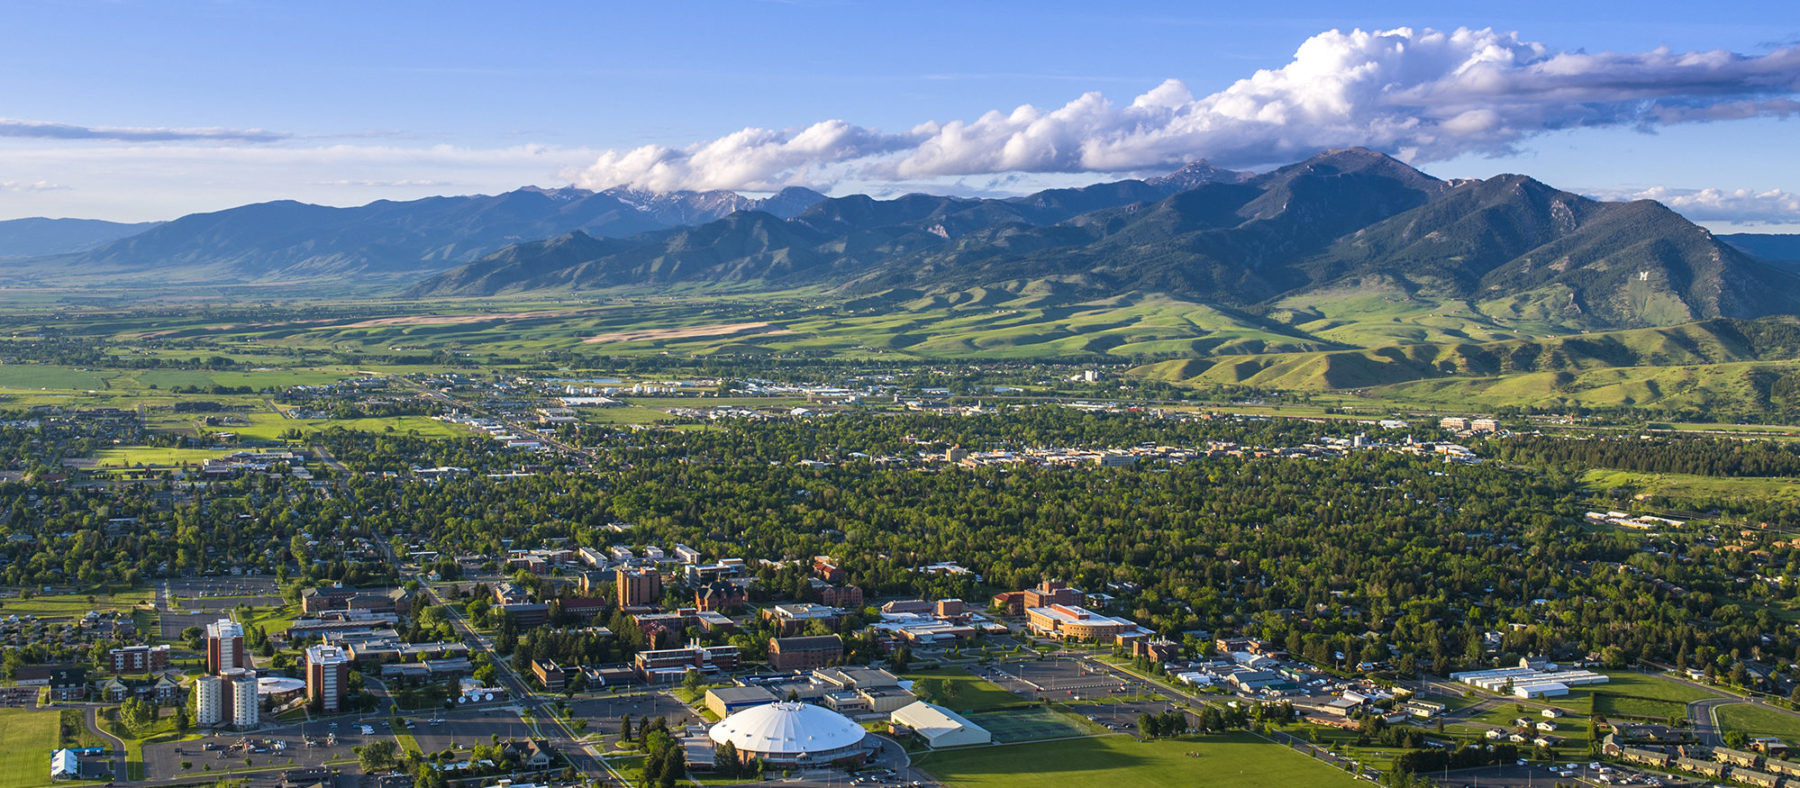
\includegraphics[width=5in,height=\textheight]{images/msu-campus.jpg}
\vspace{1cm}\\
STAT 216 Activity Coursepack}
\usepackage{etoolbox}
\makeatletter
\providecommand{\subtitle}[1]{% add subtitle to \maketitle
  \apptocmd{\@title}{\par {\large #1 \par}}{}{}
}
\makeatother
\subtitle{Fall 2020}
\author{}
\date{\vspace{-2.5em}}

\begin{document}
\maketitle

{
\setcounter{tocdepth}{0}
\tableofcontents
}
\hypertarget{preface}{%
\chapter*{Preface}\label{preface}}
\addcontentsline{toc}{chapter}{Preface}

This coursepack accompanies the textbook for STAT 216: Introduction to Statistics at Montana State University. Each of the activities in this workbook is designed to target specific learning outcomes of the course, giving you practice with important statistical concepts in a group setting with instructor guidance. Bring this workbook with you to class each week, and take notes in the workbook as you would your own notes. A well-written complete workbook will provide an optimal study guide for exams!

\hypertarget{handedness-of-male-boxers}{%
\chapter{Handedness of Male Boxers}\label{handedness-of-male-boxers}}

\hypertarget{learning-objectives}{%
\section{Learning objectives}\label{learning-objectives}}

\begin{itemize}
\item
  Identify the two possible explanations (one assuming the null hypothesis, and one assuming the alternative hypothesis) for a relationship seen in sample data
\item
  Given a research question, construct the null and alternative hypotheses
  in words and using appropriate statistical symbols
\item
  Describe and perform simulation-based hypothesis tests for a single proportion
\item
  Interpret and evaluate a p-value
\item
  Use bootstrapping to find a confidence interval for a single proportion
\end{itemize}

\hypertarget{terminology-review}{%
\section{Terminology review}\label{terminology-review}}

These are a few of the terms we will cover in today's activity.

\begin{itemize}
\item
  Parameter of Interest
\item
  Null Hypothesis
\item
  Alternative Hypothesis
\item
  Null distribuiton
\item
  p-value
\item
  Bootstrapping
\item
  Confidence Interval
\end{itemize}

To review these concepts see Chapter 5 in your textbook

\hypertarget{steps-of-the-statistical-investigation-process}{%
\section{Steps of the statistical investigation process}\label{steps-of-the-statistical-investigation-process}}

We will work through a six step process to complete a hypothesis test for a single proportion.

\begin{itemize}
\item
  \textbf{Ask a research question} that can be addressed by collecting data. What are the researchers trying to show.
\item
  \textbf{Design a study and collect data}. This step involves selecting the people or objects to be studied and how to gather relevant data on them.
\item
  \textbf{Summarize and Visualize the data}. Calculate summary statistics and create graphical plots that best represent the research question.
\item
  \textbf{Use statistical analysis methods to draw inferences from the data}. Choose an analysis technique appropriate for the data and identify the p-value. In this study, we will focus on using randomization.
\item
  \textbf{Communicate the results and answer the research question}. Using the p-value and confidence interval from the analysis, determine whether the data provide statistical evidence against the null hypothesis.
\item
  \textbf{Revisit and look forward} to point out limitations of the study and suggest new studies that could be performed to build on the findings of the study
\end{itemize}

\hypertarget{handedness-of-male-boxers-1}{%
\section{Handedness of male boxers}\label{handedness-of-male-boxers-1}}

Left-handedness is a trait that is found in about 10\% of the population. The fighting claim states that left-handed men have an advantage in competition. Past studies have shown that left-handed men are over-represented among professional fighters. In this random sample of 500 male boxers we will see if there is an over-prevalence of left-handed fighters.

\hypertarget{summary-statistics-review}{%
\subsection{Summary statistics review}\label{summary-statistics-review}}

\begin{enumerate}
\def\labelenumi{\arabic{enumi}.}
\tightlist
\item
  What are the observational units?
\end{enumerate}

\vspace{0.5in}

\begin{enumerate}
\def\labelenumi{\arabic{enumi}.}
\setcounter{enumi}{1}
\tightlist
\item
  What variable are we testing? Is it categorical or quantitative?
\end{enumerate}

\vspace{1in}

\begin{enumerate}
\def\labelenumi{\arabic{enumi}.}
\setcounter{enumi}{2}
\tightlist
\item
  What type of plot would be appropriate to visually display the data?
\end{enumerate}

\vspace{1in}

\begin{enumerate}
\def\labelenumi{\arabic{enumi}.}
\setcounter{enumi}{3}
\tightlist
\item
  Write out in context the statistic will we calculate to summarize the data.
\end{enumerate}

\vspace{0.5in}

\hypertarget{ask-a-research-question}{%
\subsection{Ask a research question}\label{ask-a-research-question}}

\begin{enumerate}
\def\labelenumi{\arabic{enumi}.}
\setcounter{enumi}{4}
\tightlist
\item
  Identify the research question for this study.
\end{enumerate}

\vspace{1in}

\hypertarget{design-a-study-and-collect-data}{%
\subsection{Design a study and collect data}\label{design-a-study-and-collect-data}}

\begin{enumerate}
\def\labelenumi{\arabic{enumi}.}
\setcounter{enumi}{5}
\tightlist
\item
  What is the target population for this study?
\end{enumerate}

\vspace{0.5in}

\begin{enumerate}
\def\labelenumi{\arabic{enumi}.}
\setcounter{enumi}{6}
\tightlist
\item
  Did the researchers use a biased or an unbiased method of selection? Explain your answer.
\end{enumerate}

\vspace{1in}

\hypertarget{summarize-and-visualize-the-data}{%
\subsection{Summarize and visualize the data}\label{summarize-and-visualize-the-data}}

\begin{verbatim}
#> Stance
#>  left-handed right-handed        Total 
#>           81          419          500
\end{verbatim}

\begin{enumerate}
\def\labelenumi{\arabic{enumi}.}
\setcounter{enumi}{7}
\tightlist
\item
  Calculate the appropriate summary statistic that represents the research question. Use appropriate notation.
\end{enumerate}

\vspace{0.5in}

\hypertarget{use-statistical-analysis-methods-to-draw-inferences-from-the-data}{%
\subsection{Use statistical analysis methods to draw inferences from the data}\label{use-statistical-analysis-methods-to-draw-inferences-from-the-data}}

When testing data we must first identify the null hypothesis. The null hypothesis is written about the parameter of interest, the true value of interest.

\begin{enumerate}
\def\labelenumi{\arabic{enumi}.}
\setcounter{enumi}{8}
\tightlist
\item
  Write out the parameter of interest. (Hint: the true proportion of\ldots.)
\end{enumerate}

\vspace{1in}

\begin{enumerate}
\def\labelenumi{\arabic{enumi}.}
\setcounter{enumi}{9}
\tightlist
\item
  We will assume that the true proportion of male boxers who are left handed is the same as the general population, 0.1. Using the parameter of interest in question 9, write out the null hypothesis in words.
\end{enumerate}

\vspace{1in}

The notation used for a true proportion is \(\pi\). Since this summarizes a population, it is a parameter. When writing the null hypothesis in notation we set the parameter equal to the null value, \(H_0: \pi = \pi_0\)

\begin{enumerate}
\def\labelenumi{\arabic{enumi}.}
\setcounter{enumi}{10}
\tightlist
\item
  Write the null hypothesis in notation using the null value of 0.1.
\end{enumerate}

\vspace{0.5in}

The alternative hypothesis is the claim to be tested and the direction is based on the research question.

\begin{enumerate}
\def\labelenumi{\arabic{enumi}.}
\setcounter{enumi}{11}
\tightlist
\item
  Based on the research question from question 5, are we testing that the parameter is greater than 0.1, less than 0.1 or different than 0.1?
\end{enumerate}

\vspace{0.5in}

\begin{enumerate}
\def\labelenumi{\arabic{enumi}.}
\setcounter{enumi}{12}
\tightlist
\item
  Write out the alternative hypothesis in words.
\end{enumerate}

\vspace{1in}

\begin{enumerate}
\def\labelenumi{\arabic{enumi}.}
\setcounter{enumi}{13}
\tightlist
\item
  Write out the alternative hypothesis in notation.
\end{enumerate}

\vspace{0.5in}

Remember that when utilizing a hypothesis test, we are evaluating two competing possibilities. For this study the \textbf{two possibilities} are either\ldots{}

\begin{itemize}
\item
  The true proportion of male boxers who are left handed is 0.1 and our results just occurred by random chance or
\item
  The true proportion of male boxers who are left handed is greater than 0.1 and our results reflect this
\end{itemize}

Notice that these two competing possibilities represent the null and alternative hypotheses.

The null distribution is created under the assumption the null hypothesis is true. In this case, we assume the true proportion of male boxers who are left handed is 0.1 so we will create 1000 different simulations of 500 boxers under this assumption.

Let's think about how to use cards to create one simulation of 500 boxers under the assumption the null hypothesis is true. Suppose blue cards represents left-handed and red cards represents right-handed.

\begin{enumerate}
\def\labelenumi{\arabic{enumi}.}
\setcounter{enumi}{14}
\tightlist
\item
  How many cards total do we need? How many blue ones? How many red ones?
\end{enumerate}

\vspace{0.5in}

\begin{enumerate}
\def\labelenumi{\arabic{enumi}.}
\setcounter{enumi}{15}
\tightlist
\item
  Next, we would mix the cards together and draw 1 card, write down if it's red or blue, and replace the card. How many times would we need to repeat this process to simulate our sample?
\end{enumerate}

\vspace{0.5in}

\begin{enumerate}
\def\labelenumi{\arabic{enumi}.}
\setcounter{enumi}{16}
\tightlist
\item
  What would we plot on the null distribution?
  \vspace{1in}
\end{enumerate}

We will use the computer to simulate 1000 simulated proportions of male boxers who are left handed for a sample size of 500 based on the assumption that the true proportion of male boxers who are left handed is 0.1. This is called the null distribution because it is created based on the assumption that the null hypothesis is true.

To use the computer simulation, we will need to enter the ``probability of success,'' ``sample size,'' ``number of repetitions,'' ``as extreme as,'' and the ``direction'' (matches the direction of the alternative hypothesis).

\begin{enumerate}
\def\labelenumi{\arabic{enumi}.}
\setcounter{enumi}{17}
\tightlist
\item
  What values should be entered into the simulation?
\end{enumerate}

\vspace{0.25in}

Probability of success:

\vspace{0.25in}

Sample size:

\vspace{0.25in}

Number of repetitions:

\vspace{0.25in}

As extreme as:

\vspace{0.25in}

Direction:

\vspace{0.25in}

\begin{center}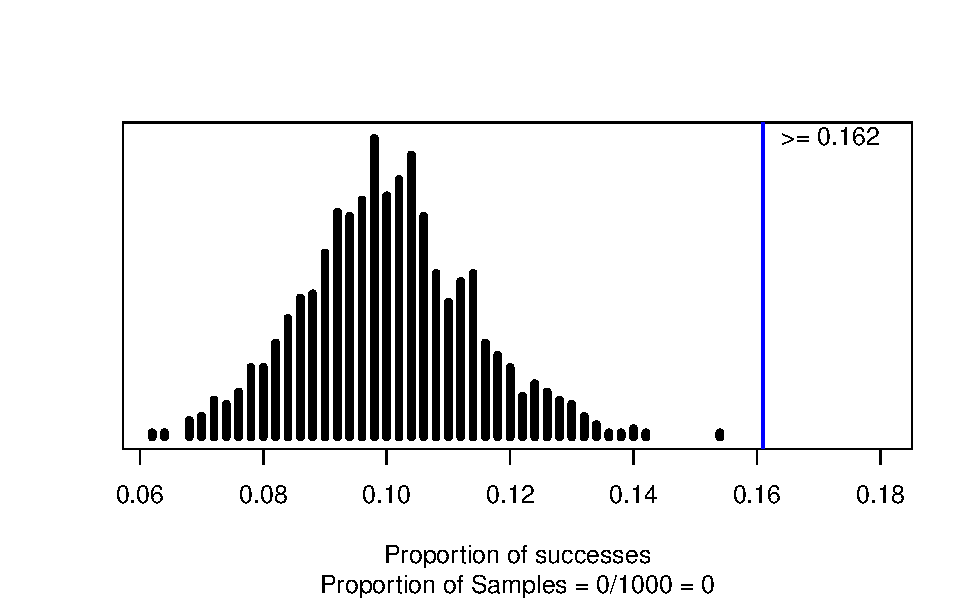
\includegraphics[width=0.7\linewidth]{06-inference-1cat_files/figure-latex/unnamed-chunk-4-1} \end{center}

\begin{enumerate}
\def\labelenumi{\arabic{enumi}.}
\setcounter{enumi}{18}
\tightlist
\item
  Around what value is the null distribution centered? Why does that make sense?
\end{enumerate}

\vspace{1in}

\begin{enumerate}
\def\labelenumi{\arabic{enumi}.}
\setcounter{enumi}{19}
\tightlist
\item
  Where does the statistic (value from question 8) fall in the null distribution? Is it towards the center or in one of the tails?
\end{enumerate}

\vspace{1in}

\begin{enumerate}
\def\labelenumi{\arabic{enumi}.}
\setcounter{enumi}{20}
\tightlist
\item
  Is the statistic likely to happen or unlikely to happen if the true proportion of male boxers is 0.1? Explain your answer.
\end{enumerate}

\vspace{1in}

\begin{enumerate}
\def\labelenumi{\arabic{enumi}.}
\setcounter{enumi}{21}
\tightlist
\item
  Using the simulation, what is the proportion of samples at this summary statistic or greater, if the true proportion of male boxers is 0.1? \emph{Hint: Look under the simulation.}
\end{enumerate}

\vspace{1in}

This is the p-value. The smaller the p-value the more evidence we have against the null hypothesis.

\begin{enumerate}
\def\labelenumi{\arabic{enumi}.}
\setcounter{enumi}{22}
\tightlist
\item
  Using the following guidelines for the strength of evidence, how much evidence do the data provide against the null hypothesis?
\end{enumerate}

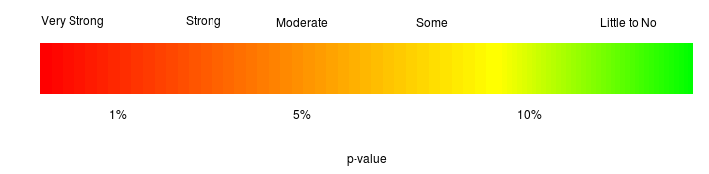
\includegraphics{images/soe_gradient.png}
\vspace{0.5in}

A point estimate provides a single plausible value for a parameter. However, a point estimate is rarely perfect; usually there is some error in the estimate. In addition to supplying a point estimate of a parameter, a next logical step would be to provide a plausible range of values for the parameter. This plausible range of values for the population parameter is called a confidence interval.

We will use bootstrapping to find the 95\% confidence interval.

\begin{enumerate}
\def\labelenumi{\arabic{enumi}.}
\setcounter{enumi}{23}
\tightlist
\item
  What is bootstrapping?
  \vspace{1in}
\end{enumerate}

\begin{center}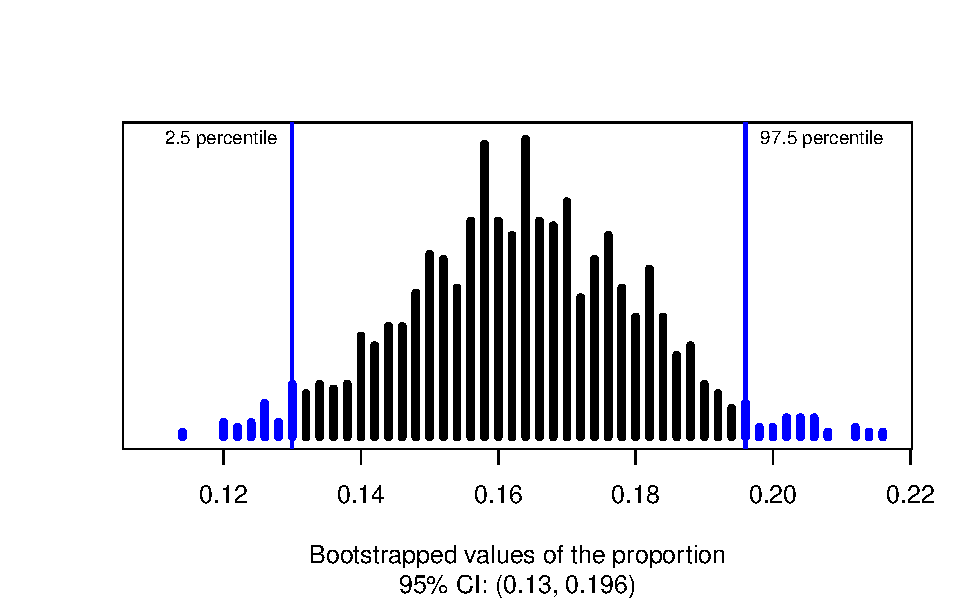
\includegraphics[width=0.7\linewidth]{06-inference-1cat_files/figure-latex/unnamed-chunk-6-1} \end{center}

\begin{enumerate}
\def\labelenumi{\arabic{enumi}.}
\setcounter{enumi}{24}
\tightlist
\item
  Explain why the blue lines are at the 2.5th percentile and the 97.5th percentile.
\end{enumerate}

\vspace{1in}

\begin{enumerate}
\def\labelenumi{\arabic{enumi}.}
\setcounter{enumi}{25}
\tightlist
\item
  Report the 95\% bootstrapped confidence interval for \(\pi\). Use interval notation: (lower value, upper value).
\end{enumerate}

\vspace{1in}

\begin{enumerate}
\def\labelenumi{\arabic{enumi}.}
\setcounter{enumi}{26}
\tightlist
\item
  What are we 95\% confident is contained within this interval?
\end{enumerate}

\vspace{1in}

\hypertarget{communicate-the-results-and-answer-the-research-question}{%
\subsection{Communicate the results and answer the research question}\label{communicate-the-results-and-answer-the-research-question}}

When we write a conclusion we answer the research question by stating how much evidence there is for the alternative hypothesis.

\begin{enumerate}
\def\labelenumi{\arabic{enumi}.}
\setcounter{enumi}{27}
\tightlist
\item
  Write a paragraph summarizing the results. Be sure to include:
\end{enumerate}

\begin{itemize}
\item
  Summary statistic
\item
  P-value
\item
  Conclusion in context
\item
  Confidence Interval
\item
  Interpretation of the Confidence Interval
\end{itemize}

\vspace{3in}

\hypertarget{revisit-and-look-forward}{%
\subsection{Revisit and look forward}\label{revisit-and-look-forward}}

\begin{enumerate}
\def\labelenumi{\arabic{enumi}.}
\setcounter{enumi}{28}
\tightlist
\item
  Suggest a new research question that you might investigate, building on what you learned in this study.
\end{enumerate}

\vspace{1in}

\hypertarget{additional-notes}{%
\section{Additional notes}\label{additional-notes}}

Use this space to summarize your thoughts and take additional notes on today's activity.

\hypertarget{helmet-use-and-head-injuries}{%
\chapter{Helmet Use and Head Injuries}\label{helmet-use-and-head-injuries}}

\hypertarget{learning-objectives}{%
\section{Learning objectives}\label{learning-objectives}}

\begin{itemize}
\item
  Write out the null and alternative hypothesis for two categorical variables
\item
  Assess the conditions to use the standard normal distributions
\item
  Calculate the Z test statistic for a difference in proportions
\item
  Find the p-value and assess the strength of evidence
\item
  Create and interpret a confidence interval for the difference in proportions
\end{itemize}

\hypertarget{terminology-review}{%
\section{Terminology review}\label{terminology-review}}

Here are a few terms we will use in today's activity.

\begin{itemize}
\item
  Conditional proportion
\item
  Z test
\item
  z* multiplier
\item
  Null Hypothesis
\item
  Alternative Hypothesis
\item
  Test statistic
\end{itemize}

Review Chapter 5 in your textbook for more information on these topics.

\hypertarget{helmet-use-and-head-injuries-1}{%
\section{Helmet Use and Head Injuries}\label{helmet-use-and-head-injuries-1}}

In ``Helmet Use and Risk of Head Injuries in Alpine Skiers and Snowboarders'' by Sullheim et. al., in the Journal of the American Medical Association, Vol. 295, No.~8, we can see the results from a random sample 3562 skiers and snowboarders involved in accidents.

\begin{longtable}[]{@{}llll@{}}
\toprule
& Head Injury & No Head Injury & Total\tabularnewline
\midrule
\endhead
Wore Helmet & 96 & 656 & 752\tabularnewline
Did Not Wear Helmet & 480 & 2330 & 2810\tabularnewline
Total & 576 & 2986 & 3562\tabularnewline
\bottomrule
\end{longtable}

Is there evidence that safety helmet use reduces the risk of head injury for skiers and snowboarders?

\hypertarget{vocabulary-review}{%
\subsection{Vocabulary review}\label{vocabulary-review}}

\begin{enumerate}
\def\labelenumi{\arabic{enumi}.}
\tightlist
\item
  What is the explanatory variable?
\end{enumerate}

\vspace{0.5in}

\begin{enumerate}
\def\labelenumi{\arabic{enumi}.}
\setcounter{enumi}{1}
\tightlist
\item
  What is the response variable?
\end{enumerate}

\vspace{0.5in}

\begin{enumerate}
\def\labelenumi{\arabic{enumi}.}
\setcounter{enumi}{2}
\tightlist
\item
  Is this an experiment or observational study?
\end{enumerate}

\vspace{0.5in}

\begin{enumerate}
\def\labelenumi{\arabic{enumi}.}
\setcounter{enumi}{3}
\tightlist
\item
  Put an X in the box that represents the appropriate scope of inference for this study.
\end{enumerate}

\begin{longtable}[]{@{}cccl@{}}
\toprule
& & Study Type &\tabularnewline
\midrule
\endhead
& & Randomized Experiment & Observational Study\tabularnewline
Selection of Cases & Random Sample & &\tabularnewline
& No Random Sample & &\tabularnewline
\bottomrule
\end{longtable}

\begin{enumerate}
\def\labelenumi{\arabic{enumi}.}
\setcounter{enumi}{4}
\tightlist
\item
  What is the conditional proportion of skiers/snowboarders with a head injury that wore a helmet?
\end{enumerate}

\vspace{1in}

\begin{enumerate}
\def\labelenumi{\arabic{enumi}.}
\setcounter{enumi}{5}
\tightlist
\item
  What is the conditional proportion of skiers/snowboarders with a head injury that did not wear a helmet?
\end{enumerate}

\vspace{1in}

\hypertarget{ask-a-research-question}{%
\subsection{Ask a research question}\label{ask-a-research-question}}

In this study we are looking at the relationship between two groups or two parameters (\(\pi_1\) and \(\pi_2\)). Remember we define the parameter as the true proportion of observational units that represent the variable of interest.

\begin{enumerate}
\def\labelenumi{\arabic{enumi}.}
\setcounter{enumi}{6}
\tightlist
\item
  What is the variable of interest in this study?
\end{enumerate}

\vspace{0.5in}

\begin{enumerate}
\def\labelenumi{\arabic{enumi}.}
\setcounter{enumi}{7}
\item
  Write the two parameters of interest for this study. Let 1 = skier/snowboarder wore helmet, 2 = skier/snowboarder did not wear helmet.

  \(\pi_1\) -
  \vspace{0.5in}

  \(\pi_2\) -
  \vspace{0.5in}
\end{enumerate}

When comparing two groups, we assume the two parameters are equal in the null hypothesis. There is no association between the variables.

\begin{enumerate}
\def\labelenumi{\arabic{enumi}.}
\setcounter{enumi}{8}
\tightlist
\item
  Write the null hypothesis out in words using your answers to question 8.
\end{enumerate}

\vspace{1in}

\begin{enumerate}
\def\labelenumi{\arabic{enumi}.}
\setcounter{enumi}{9}
\tightlist
\item
  What is the research question?
\end{enumerate}

\vspace{1in}

\begin{enumerate}
\def\labelenumi{\arabic{enumi}.}
\setcounter{enumi}{10}
\tightlist
\item
  Based on the research question fill in the appropriate sign for the alternative hypothesis:
  \vspace{0.25in}
\end{enumerate}

\(H_A: \pi_1 -\pi_2\) \_\_\_\_\_\_\_\_\_\_ 0

\hypertarget{summarize-and-visualize-the-data}{%
\subsection{Summarize and visualize the data}\label{summarize-and-visualize-the-data}}

\begin{center}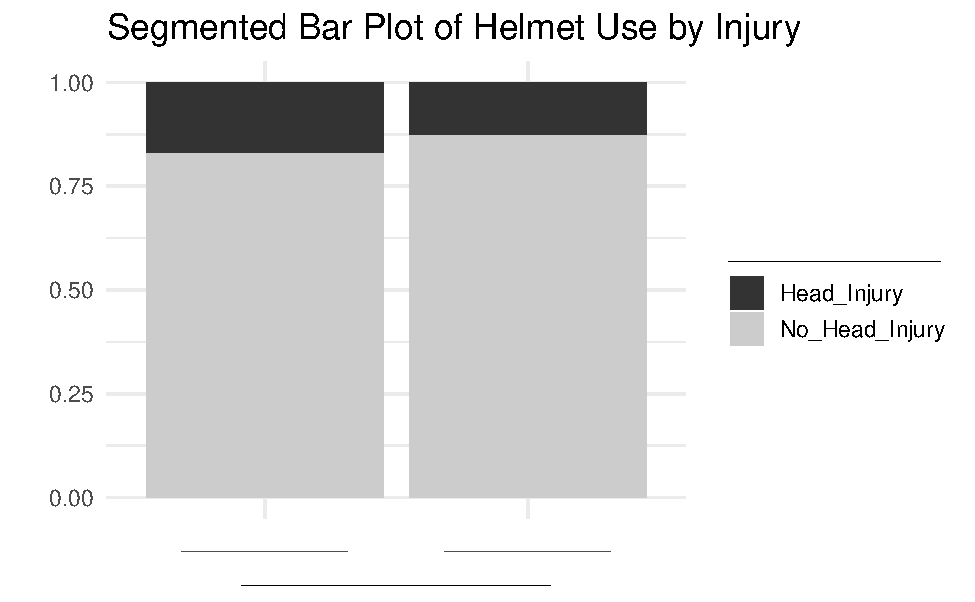
\includegraphics[width=0.7\linewidth]{07-inference-2cat_files/figure-latex/unnamed-chunk-2-1} \end{center}

\begin{enumerate}
\def\labelenumi{\arabic{enumi}.}
\setcounter{enumi}{11}
\tightlist
\item
  Fill in the blanks on the graph with the appropriate variables and values to plot a segmented bar plot of injury by helmet use.
\end{enumerate}

\vspace{1in}

\begin{enumerate}
\def\labelenumi{\arabic{enumi}.}
\setcounter{enumi}{12}
\tightlist
\item
  Based on the bar plot, Does there appear to be an association between helmet use and head injury? Explain.
\end{enumerate}

\vspace{1in}

\begin{enumerate}
\def\labelenumi{\arabic{enumi}.}
\setcounter{enumi}{13}
\tightlist
\item
  Calculate the point estimate for this study. We will use helmet use minus no helmet use as the order of subtraction.
\end{enumerate}

\vspace{1in}

\begin{enumerate}
\def\labelenumi{\arabic{enumi}.}
\setcounter{enumi}{14}
\tightlist
\item
  What is the notation used for the value calculated in question 14?
\end{enumerate}

\vspace{0.5in}

\hypertarget{use-statistical-analysis-methods-to-draw-inferences-from-the-data}{%
\subsection{Use statistical analysis methods to draw inferences from the data}\label{use-statistical-analysis-methods-to-draw-inferences-from-the-data}}

To test the null hypothesis we could use simulation methods as we did with a single categorical variable. In this activity we will focus on theory-based methods. Like with a single proportion, the difference in proportions can be mathematically modeled using the normal distribution if certain conditions are met.

Conditions for the sample distribution of \(\hat{p}_1-\hat{p}_2\)

\begin{itemize}
\item
  Independence: The data are independent within and between the two groups.
\item
  Success-Failure Condition: The success-failure condition holds for each group.
\end{itemize}

\vspace{.25in}

\begin{enumerate}
\def\labelenumi{\arabic{enumi}.}
\setcounter{enumi}{15}
\tightlist
\item
  Is the independence condition met? Explain your answer.
\end{enumerate}

\vspace{1in}

\begin{enumerate}
\def\labelenumi{\arabic{enumi}.}
\setcounter{enumi}{16}
\tightlist
\item
  Is the success-failure condition met for each group? Explain your answer.
\end{enumerate}

\vspace{1in}

To calculate the test statistic we use:

\begin{center}
    $Z = \frac{\text{point estimate} - \text{null value}}{SE}$

where the standard error is calculated using the pooled proportion of successes.

   $SE(\hat{p}_1-\hat{p}_2)=\sqrt{\hat{p}_{pool}(1-\hat{p}_{pool})(\frac{1}{n_1}+\frac{1}{n_2})}, \text{where}$ 
    
   $\hat{p}_{pool} = \frac{\text{number of "successes"}}{\text{number of cases}} = \frac{\hat{p}_1 n_1+\hat{p}_2 n_2}{n_1+n_2}$
    
\end{center}

\vspace{.25in}

\begin{enumerate}
\def\labelenumi{\arabic{enumi}.}
\setcounter{enumi}{17}
\tightlist
\item
  Calculate the \(SE(\hat{p}_1-\hat{p}_2)\).
\end{enumerate}

\vspace{1in}

\begin{enumerate}
\def\labelenumi{\arabic{enumi}.}
\setcounter{enumi}{18}
\tightlist
\item
  Calculate the test statistic.
\end{enumerate}

\vspace{1in}

We will use the pnorm function in R to find the p-value.

\begin{verbatim}
#> [1] 0.002118205
\end{verbatim}

\begin{enumerate}
\def\labelenumi{\arabic{enumi}.}
\setcounter{enumi}{19}
\item
  Report the p-value.
  \vspace{0.5in}
\item
  How much evidence does the p-value provide against the null hypothesis?
\end{enumerate}

\vspace{0.5in}

To find a confidence interval for the difference in proportions we will add and subtract the margin of error from the point estimate to find the two endpoints.

\[\hat{p}_1-\hat{p}_2\pm z^*SE(\hat{p}_1-\hat{p}_2), \text{where}\]

\[SE(\hat{p}_1-\hat{p}_2) = \sqrt{\left(\frac{\hat{p}_1 (1-\hat{p}_1)}{n_1}+\frac{\hat{p}_2 (1-\hat{p}_2)}{n_2}\right)}\]

Note that the formula changes when calculating the variability around the statistic in order to calculate a confidence interval! Here use the sample proportions for each group to calculate the standard error for the difference in proportions. The \(z^*\) multiplier is found under the normal distribution. We find the values that encompass the middle 95\% of the data.

\begin{verbatim}
#> [1] 1.959964
\end{verbatim}

\begin{enumerate}
\def\labelenumi{\arabic{enumi}.}
\setcounter{enumi}{21}
\tightlist
\item
  Calculate the standard error for a difference in proportions to create a 95\% confidence interval.
\end{enumerate}

\vspace{1in}

\begin{enumerate}
\def\labelenumi{\arabic{enumi}.}
\setcounter{enumi}{22}
\tightlist
\item
  Using the multiplier of \(z^*\) = 1.96, calculate the 95\% confidence interval for the difference in true proportion of head injuries for those that used helmets minus those who did not.
\end{enumerate}

\vspace{1in}

\begin{enumerate}
\def\labelenumi{\arabic{enumi}.}
\setcounter{enumi}{23}
\tightlist
\item
  Interpret the confidence interval found in question 23 in context of the problem.
\end{enumerate}

\vspace{1in}

\begin{enumerate}
\def\labelenumi{\arabic{enumi}.}
\setcounter{enumi}{24}
\tightlist
\item
  Write a paragraph summarizing the results of the study. Be sure to include:
\end{enumerate}

\begin{itemize}
\item
  Summary statistic
\item
  P-value
\item
  Conclusion (written to answer the research question)
\item
  Confidence interval
\item
  Interpretation of the confidence interval
\item
  Scope of inference
\end{itemize}

\vspace{3in}

\hypertarget{types-of-errors}{%
\subsection{Types of errors}\label{types-of-errors}}

Hypothesis tests are not flawless. In a hypothesis test, there are two competing hypotheses: the null and alternative. We make a decision about which might be true, but we may choose incorrectly.

\begin{longtable}[]{@{}ccll@{}}
\toprule
& & Test Conclusion &\tabularnewline
\midrule
\endhead
Truth & \(H_0\) true & good decision & Type 1 Error\tabularnewline
& \(H_A\) true & Type 2 Error & good decision\tabularnewline
\bottomrule
\end{longtable}

A Type 1 Error is rejecting the null hypothesis when \(H_0\)is actually true. A Type 2 Error is failing to reject the null hypothesis when the alternative is actually true.

\begin{enumerate}
\def\labelenumi{\arabic{enumi}.}
\setcounter{enumi}{25}
\tightlist
\item
  Using a significance level of 0.05, what decision do you make in regards to the null hypothesis?
\end{enumerate}

\vspace{0.5in}

\begin{enumerate}
\def\labelenumi{\arabic{enumi}.}
\setcounter{enumi}{26}
\tightlist
\item
  What type of error could we have made?
\end{enumerate}

\vspace{0.5in}

\begin{enumerate}
\def\labelenumi{\arabic{enumi}.}
\setcounter{enumi}{27}
\tightlist
\item
  Write this error in context of the problem.
\end{enumerate}

\vspace{1in}

\hypertarget{additional-notes}{%
\section{Additional notes}\label{additional-notes}}

Use this space to summarize your thoughts and take additional notes on today's activity.

\hypertarget{covid-19-and-air-pollution}{%
\chapter{COVID-19 and Air Pollution}\label{covid-19-and-air-pollution}}

\hypertarget{learning-outcomes}{%
\section{Learning outcomes}\label{learning-outcomes}}

\begin{itemize}
\item
  Given a research question, construct the null and alternative hypotheses
  in words and using appropriate statistical symbols
\item
  Describe and perform simulation-based hypothesis for paired quantitative data
\item
  Interpret and evaluate a p-value
\item
  Find a confidence interval for the mean difference using bootstrapping
\item
  Use a confidence interval to determine the conclusion of a hypothesis test
\end{itemize}

\hypertarget{terminology-review}{%
\section{Terminology review}\label{terminology-review}}

The following terms will be covered in this activity.

\begin{itemize}
\item
  Mean difference
\item
  Paired data
\item
  Independent groups
\item
  Shifted Null Distribution
\end{itemize}

For further explanation of these topics see Section 6.2 in the textbook.

\hypertarget{covid-19-and-air-pollution-1}{%
\section{COVID-19 and air pollution}\label{covid-19-and-air-pollution-1}}

The social distancing efforts and stay-at-home directives to help combat the spread of COVID-19 have appeared to help `flatten the curve' across the United States, albeit at a high cost to many individuals and businesses. The impact of these measures, though, goes far beyond the infection and death rates from the disease. You may have seen images comparing air quality in large international cities like Rome, Milan, Wuhan, and New Delhi such as the one pictured below which seem to indicate, perhaps unsurprisingly, that fewer people driving and factories being shut down have reduced air pollutants.

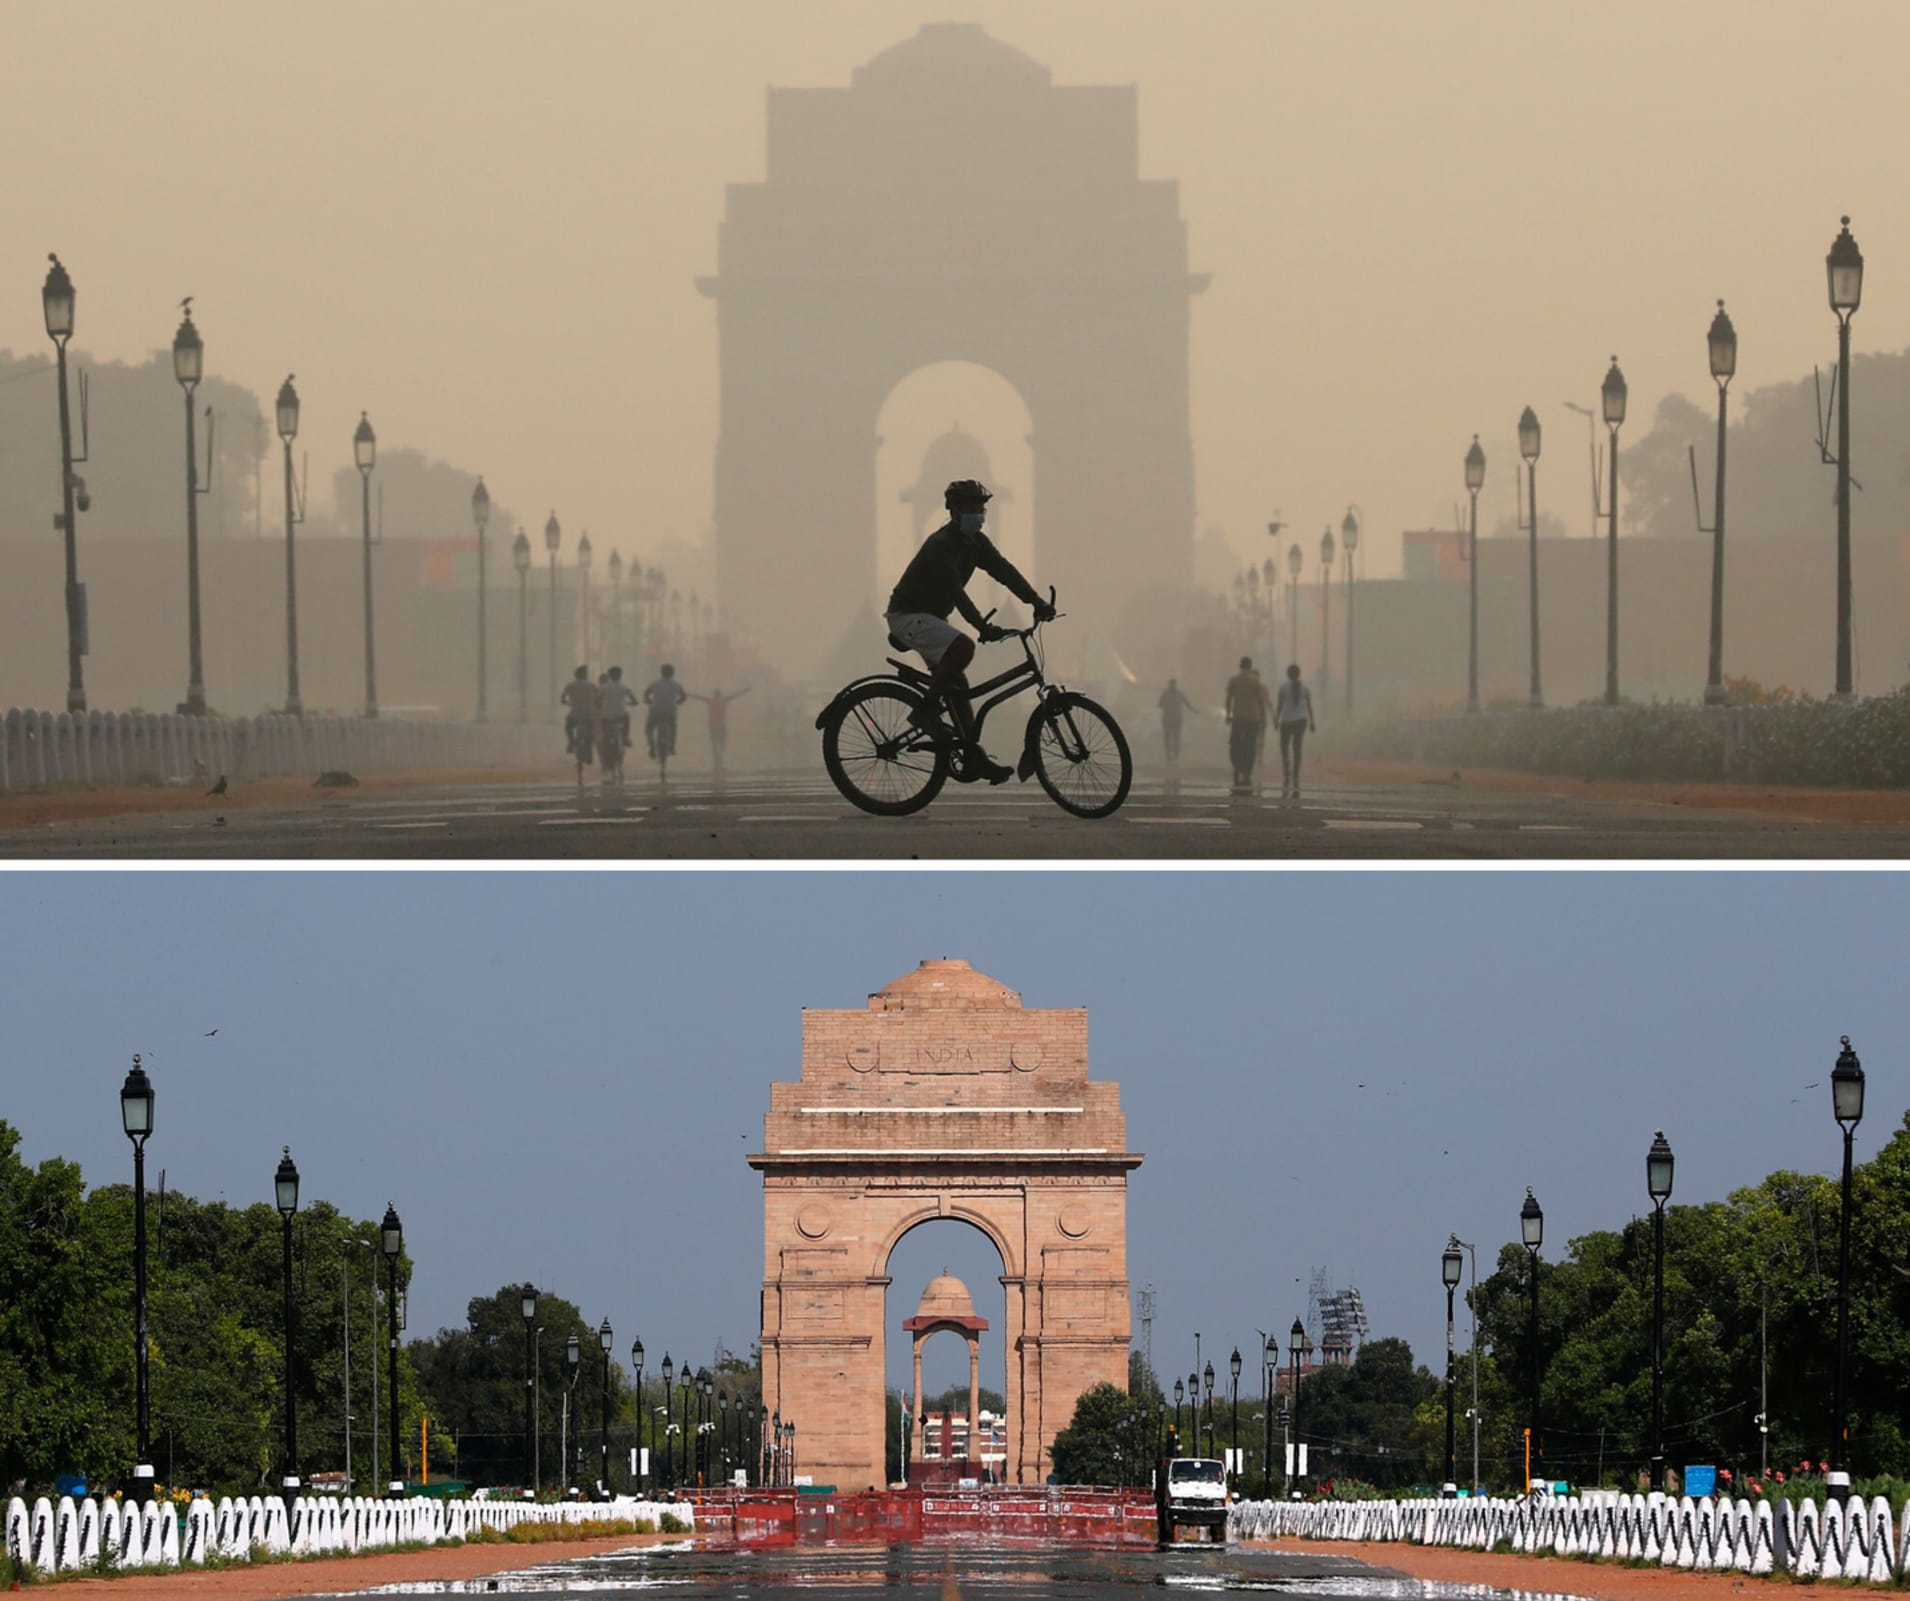
\includegraphics{images/air_pollution.png}

Have high population-density U.S. cities seen the same improved air quality conditions? To study this question, data was gathered from the U.S. Environmental Protection Agency (EPA) AirData website which records the ozone (O3) and fine particulate matter (PM2.5) values for cities across the U.S. These measures are used to calculate an air quality index (AQI) score for each city each day of the year. Thirty-three of the most densely populated U.S. cities were selected and the AQI score recorded for April 20, 2020 as well as the five-year median AQI score for April 20th (2015 - 2019). Note that higher AQI scores indicate worse air quality.

\hypertarget{vocabulary-review}{%
\subsection{Vocabulary review}\label{vocabulary-review}}

\begin{center}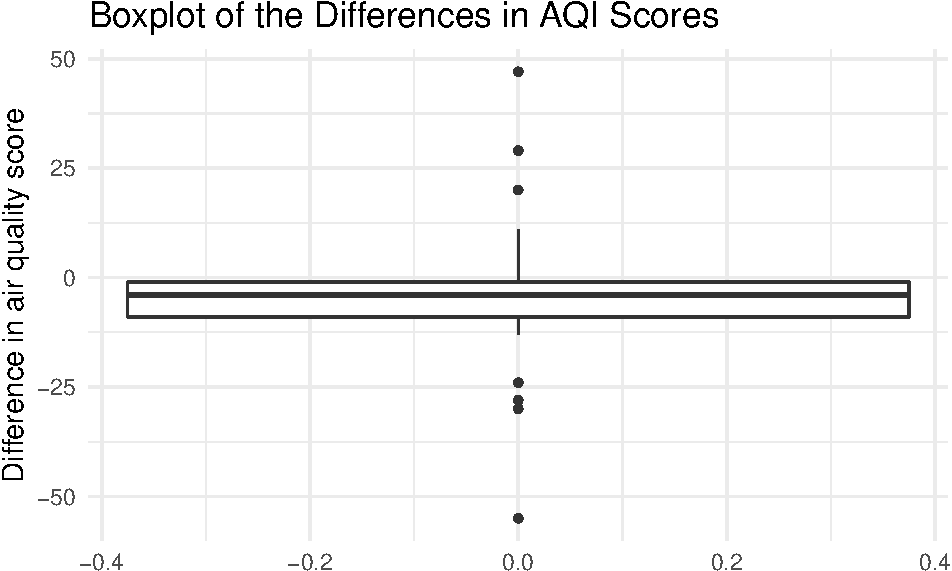
\includegraphics[width=0.7\linewidth]{08-paired_files/figure-latex/unnamed-chunk-2-1} \end{center}

\begin{longtable}[]{@{}ccll@{}}
\toprule
& Mean & Standard deviation & Sample Size\tabularnewline
\midrule
\endhead
Current & \(\bar{x}_1\) = 47.394 & \(s_1\) = 14.107 & \(n_1\) = 33\tabularnewline
5 Year Median & \(\bar{x}_2\) = 51.545 & \(s_2\) = 17.447 & \(n_2\) = 33\tabularnewline
Differences & \(\bar{x}_d\) = -4.152 & \(s_d\) = 17.096 & \(n_d\) = 33\tabularnewline
\bottomrule
\end{longtable}

\begin{enumerate}
\def\labelenumi{\arabic{enumi}.}
\tightlist
\item
  What is the sample size?
\end{enumerate}

\vspace{0.5in}

\begin{enumerate}
\def\labelenumi{\arabic{enumi}.}
\setcounter{enumi}{1}
\tightlist
\item
  Identify the variables in this study. What role do each have?
\end{enumerate}

\vspace{1in}

\begin{enumerate}
\def\labelenumi{\arabic{enumi}.}
\setcounter{enumi}{2}
\tightlist
\item
  Why is this treated as a paired study design and not two independent samples?
\end{enumerate}

\vspace{1in}

\begin{enumerate}
\def\labelenumi{\arabic{enumi}.}
\setcounter{enumi}{3}
\tightlist
\item
  Is this an experiment or observational study?
\end{enumerate}

\vspace{0.5in}

\hypertarget{ask-a-research-question}{%
\subsection{Ask a research question}\label{ask-a-research-question}}

\begin{enumerate}
\def\labelenumi{\arabic{enumi}.}
\setcounter{enumi}{4}
\tightlist
\item
  What are the two competing possibilities to run a hypothesis test?
\end{enumerate}

\vspace{1in}

\begin{enumerate}
\def\labelenumi{\arabic{enumi}.}
\setcounter{enumi}{5}
\tightlist
\item
  Write the null hypothesis in words.
\end{enumerate}

\vspace{1in}

\begin{enumerate}
\def\labelenumi{\arabic{enumi}.}
\setcounter{enumi}{6}
\tightlist
\item
  What is the research question?
\end{enumerate}

\vspace{1in}

\begin{enumerate}
\def\labelenumi{\arabic{enumi}.}
\setcounter{enumi}{7}
\tightlist
\item
  Write the alternative hypothesis in notation.
\end{enumerate}

\vspace{1in}

\hypertarget{summarize-and-visualize-the-data}{%
\subsection{Summarize and visualize the data}\label{summarize-and-visualize-the-data}}

\begin{enumerate}
\def\labelenumi{\arabic{enumi}.}
\setcounter{enumi}{8}
\tightlist
\item
  Report the summary statistic for the data.
\end{enumerate}

\vspace{0.5in}

\begin{enumerate}
\def\labelenumi{\arabic{enumi}.}
\setcounter{enumi}{9}
\tightlist
\item
  What notation is used for the value in question 9?
\end{enumerate}

\vspace{0.5in}

\hypertarget{use-statistical-inferential-methods-to-draw-inferences-from-the-data}{%
\subsection{Use statistical inferential methods to draw inferences from the data}\label{use-statistical-inferential-methods-to-draw-inferences-from-the-data}}

To simulate the null distribution we will use a bootstrapping method - sampling with replacement from the data set. Before bootstrapping we will need to shift the each data point by the difference \(\mu_0 - \bar{x}\). This will ensure that the simulated null distribution will be centered at the null value.

\begin{enumerate}
\def\labelenumi{\arabic{enumi}.}
\setcounter{enumi}{10}
\tightlist
\item
  Calculate the difference \(\mu_0 - \bar{x}\). Will we need to shift the data up or down?
\end{enumerate}

\vspace{1in}

The image below gives the null distribution from one possible set of 1000 bootstrap samples:

\begin{center}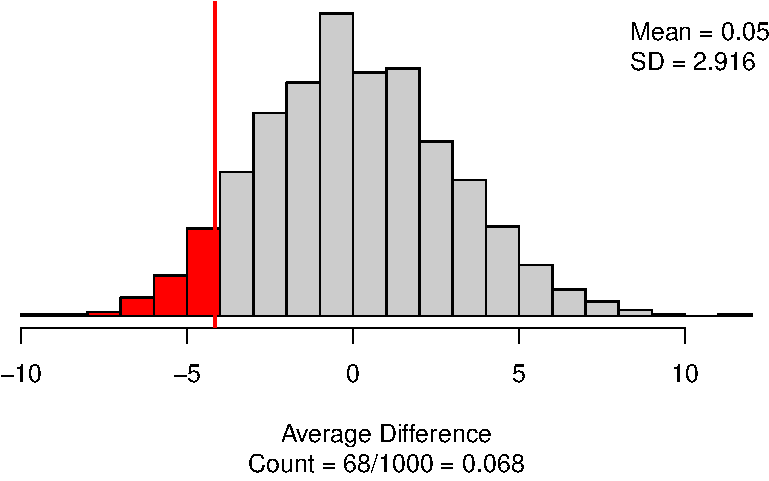
\includegraphics[width=0.7\linewidth]{08-paired_files/figure-latex/unnamed-chunk-4-1} \end{center}

\begin{enumerate}
\def\labelenumi{\arabic{enumi}.}
\setcounter{enumi}{11}
\tightlist
\item
  Explain why the null distribution is centered at zero.
\end{enumerate}

\vspace{1in}

\begin{enumerate}
\def\labelenumi{\arabic{enumi}.}
\setcounter{enumi}{12}
\tightlist
\item
  What proportion of samples are beyond the sample mean difference in AQI Scores for current scores minus 5 year median scores?
\end{enumerate}

\vspace{1in}

\begin{enumerate}
\def\labelenumi{\arabic{enumi}.}
\setcounter{enumi}{13}
\tightlist
\item
  Interpret the p-value in the context of the problem.
\end{enumerate}

\vspace{1in}

\begin{enumerate}
\def\labelenumi{\arabic{enumi}.}
\setcounter{enumi}{14}
\tightlist
\item
  How much evidence does this provide for improved air quality in US cities?
\end{enumerate}

\vspace{1in}

\begin{enumerate}
\def\labelenumi{\arabic{enumi}.}
\setcounter{enumi}{15}
\tightlist
\item
  Write out the parameter of interest in context of the study.
\end{enumerate}

\vspace{1in}

\begin{center}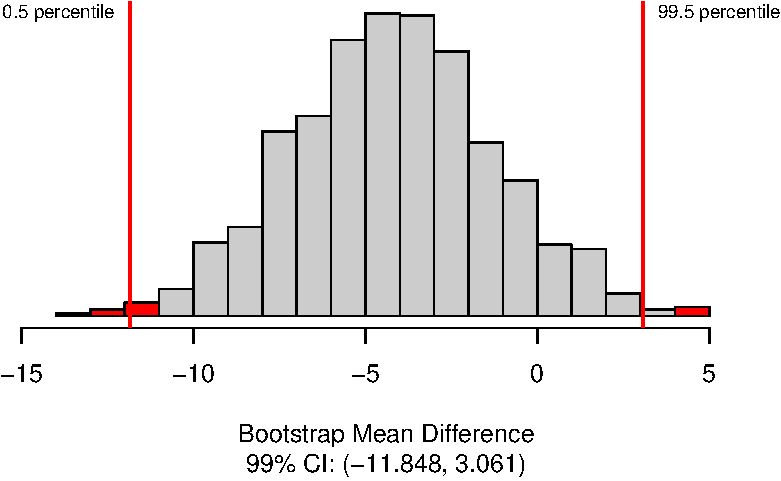
\includegraphics[width=0.7\linewidth]{08-paired_files/figure-latex/unnamed-chunk-5-1} \end{center}

\begin{enumerate}
\def\labelenumi{\arabic{enumi}.}
\setcounter{enumi}{16}
\tightlist
\item
  Use bootstrapping to find a 99\% confidence interval for the parameter of interest. Fill in the data, number of bootstrap samples, and confidence level. Report the confidence interval in interval notation.
\end{enumerate}

\vspace{1in}

\hypertarget{communicate-the-results-and-answer-the-research-question.}{%
\subsection{Communicate the results and answer the research question.}\label{communicate-the-results-and-answer-the-research-question.}}

\begin{enumerate}
\def\labelenumi{\arabic{enumi}.}
\setcounter{enumi}{17}
\tightlist
\item
  Interpret the 99\% confidence interval in the following figure in the context of the problem.
\end{enumerate}

\vspace{1in}

\begin{enumerate}
\def\labelenumi{\arabic{enumi}.}
\setcounter{enumi}{18}
\tightlist
\item
  Write a paragraph summarizes the results of this study. Be sure to include:
\end{enumerate}

\begin{itemize}
\item
  Summary statistic
\item
  P-value
\item
  Interpretation of the p-value
\item
  Confidence Interval
\item
  Interpretation of the confidence interval
\item
  Conclusion in context
\end{itemize}

\vspace{3in}

\hypertarget{revisit-and-look-forward}{%
\subsection{Revisit and look forward}\label{revisit-and-look-forward}}

\hypertarget{additional-notes}{%
\section{Additional notes}\label{additional-notes}}

Use this space to summarize your thoughts and take additional notes on today's activity.

\hypertarget{record-snowfall}{%
\chapter{Record Snowfall}\label{record-snowfall}}

\hypertarget{learning-objectives}{%
\section{Learning objectives}\label{learning-objectives}}

\begin{itemize}
\item
  Write out the null and alternative hypothesis for one categorical and one quantitative Variable
\item
  Calculate and carry-out simulation based hypothesis test for a difference in means
\item
  Interpret and evaluate a p-value
\item
  Find a bootstap confidence interval for the difference in means
\item
  Use a confidence interval to determine the conclusion of a hypothesis test
\end{itemize}

\hypertarget{record-snowfall-1}{%
\section{Record snowfall}\label{record-snowfall-1}}

In the winter of 2018-2019, Bozeman had a record snowfall which resulted in the collapse of two flat-roofed buildings on the MSU campus. A writer for the Washington Post predicted the heavy snowfall for 2018-2019 due to the El Nino weather pattern that occurred in that season. A meteorologist in Montana wanted to see if the weather pattern really was associated with total snowfall. She obtained historical data from 44 years on the weather pattern (El Nino or La Nina) and snowfall (in inches) at the Billings Weather Station.

\begin{Shaded}
\begin{Highlighting}[]
\KeywordTok{favstats}\NormalTok{(Snowfall}\OperatorTok{\textasciitilde{}}\NormalTok{WeatherPattern, }\DataTypeTok{data=}\NormalTok{Snow)}
\CommentTok{\#\textgreater{}   WeatherPattern  min   Q1 median   Q3   max     mean       sd  n missing}
\CommentTok{\#\textgreater{} 1        El\_Nino 31.9 46.4   57.7 64.3  87.9 56.23043 13.00823 23       0}
\CommentTok{\#\textgreater{} 2        La\_Nina 44.5 51.4   60.9 70.3 107.2 63.13333 15.48626 21       0}
\end{Highlighting}
\end{Shaded}

\begin{Shaded}
\begin{Highlighting}[]
\KeywordTok{ggplot}\NormalTok{(}\DataTypeTok{data =}\NormalTok{ Snow,}
       \KeywordTok{aes}\NormalTok{(}\DataTypeTok{x =}\NormalTok{ WeatherPattern, }\DataTypeTok{y =}\NormalTok{ Snowfall)) }\OperatorTok{+}
\StringTok{    }\KeywordTok{geom\_boxplot}\NormalTok{() }\OperatorTok{+}\StringTok{ }
\StringTok{    }\KeywordTok{labs}\NormalTok{(}\DataTypeTok{title =} \StringTok{"Snowfall by weather pattern"}\NormalTok{,}
         \DataTypeTok{x =} \StringTok{"Weather pattern"}\NormalTok{)}
\end{Highlighting}
\end{Shaded}

\begin{center}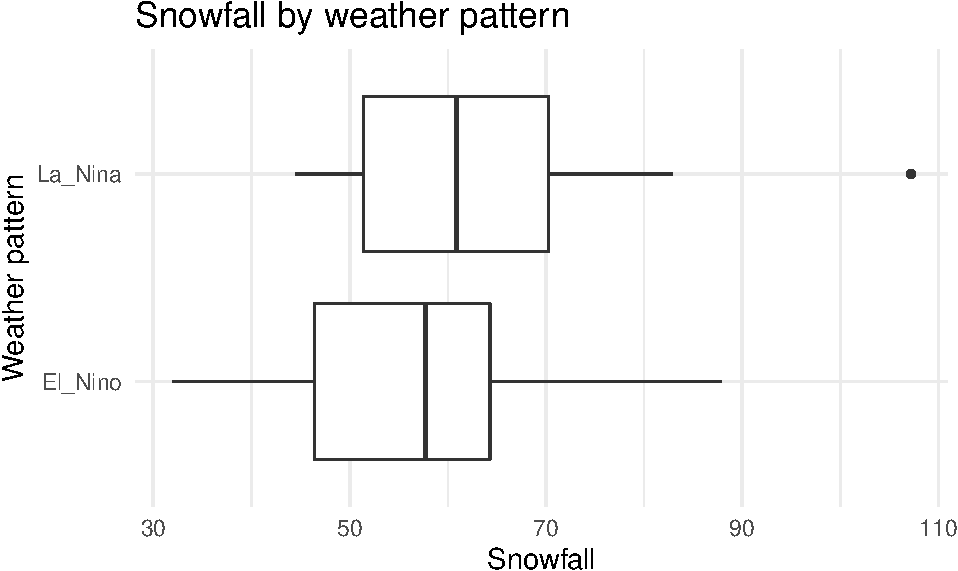
\includegraphics[width=0.7\linewidth]{09-inference-2quant_files/figure-latex/unnamed-chunk-3-1} \end{center}

\hypertarget{quantitative-variables-review}{%
\subsection{Quantitative variables review}\label{quantitative-variables-review}}

\begin{enumerate}
\def\labelenumi{\arabic{enumi}.}
\tightlist
\item
  The two variables assessed in this study are the type of weather pattern and snowfall. Identify the role for each variable (explanatory, response).
\end{enumerate}

\vspace{1in}

\begin{enumerate}
\def\labelenumi{\arabic{enumi}.}
\setcounter{enumi}{1}
\tightlist
\item
  Which group (El Nino or La Nina) has the highest center? Explain what measure you are using?
\end{enumerate}

\vspace{1in}

\begin{enumerate}
\def\labelenumi{\arabic{enumi}.}
\setcounter{enumi}{2}
\tightlist
\item
  Using the side-by-side boxplots, which group has the largest spread? How did you make that choice?
\end{enumerate}

\vspace{1in}

\begin{enumerate}
\def\labelenumi{\arabic{enumi}.}
\setcounter{enumi}{3}
\tightlist
\item
  Is this an experiment or an observational study? Explain your reasoning.
\end{enumerate}

\vspace{1in}

\begin{enumerate}
\def\labelenumi{\arabic{enumi}.}
\setcounter{enumi}{4}
\tightlist
\item
  Is this a paired data set or independent groups? Explain your answer.
\end{enumerate}

\vspace{1in}

\hypertarget{ask-a-research-question.}{%
\subsection{Ask a research question.}\label{ask-a-research-question.}}

\begin{enumerate}
\def\labelenumi{\arabic{enumi}.}
\setcounter{enumi}{5}
\tightlist
\item
  Write out the parameter of interest in context of the study. Use proper notation and be sure to define your subscripts. Use El Nino minus La Nina as the order of subtraction.
\end{enumerate}

\vspace{1in}

\begin{enumerate}
\def\labelenumi{\arabic{enumi}.}
\setcounter{enumi}{6}
\tightlist
\item
  What are the two competing possibilities we will evaluate in this study?
\end{enumerate}

\vspace{1in}

\begin{enumerate}
\def\labelenumi{\arabic{enumi}.}
\setcounter{enumi}{7}
\tightlist
\item
  Identify which is the null hypothesis and which is the alternative hypothesis.
\end{enumerate}

\vspace{1in}

\hypertarget{summarize-and-visualize-the-data}{%
\subsection{Summarize and visualize the data}\label{summarize-and-visualize-the-data}}

\begin{enumerate}
\def\labelenumi{\arabic{enumi}.}
\setcounter{enumi}{8}
\tightlist
\item
  Calculate the summary statistic. Use El Nino minus La Nina as the order of subtraction. What is the appropriate notation for the statistic?
\end{enumerate}

\vspace{0.5in}

\hypertarget{use-statistical-inferential-methods-to-draw-inferences-from-the-data}{%
\subsection{Use statistical inferential methods to draw inferences from the data}\label{use-statistical-inferential-methods-to-draw-inferences-from-the-data}}

Remember that the null distribution is created based on the assumption the null hypothesis is true. In this study, we asssume there is no association between variables. This means that a snowfall value could be in either an El Nino year or a La Nina year.

To demonstrate this your instructor will use cards to represent the sample.

\begin{enumerate}
\def\labelenumi{\arabic{enumi}.}
\setcounter{enumi}{9}
\tightlist
\item
  How many cards will we start with?
\end{enumerate}

\vspace{0.5in}

\begin{enumerate}
\def\labelenumi{\arabic{enumi}.}
\setcounter{enumi}{10}
\tightlist
\item
  What will we write on each card?
\end{enumerate}

\vspace{0.5in}

\begin{enumerate}
\def\labelenumi{\arabic{enumi}.}
\setcounter{enumi}{11}
\tightlist
\item
  Next we will mix the cards together and shuffle into two piles. How many cards will go into each pile? What should we label the piles?
\end{enumerate}

\vspace{1in}

\begin{enumerate}
\def\labelenumi{\arabic{enumi}.}
\setcounter{enumi}{12}
\tightlist
\item
  What value is calculated from the cards and plotted on the null distribution?
\end{enumerate}

\vspace{1in}

\begin{enumerate}
\def\labelenumi{\arabic{enumi}.}
\setcounter{enumi}{13}
\tightlist
\item
  Once we create a null distribution of 1000 simulations, at what value do you expect the distribution to be centered at? Explain your answer.
\end{enumerate}

\vspace{1in}

\textbf{simulation}

\begin{enumerate}
\def\labelenumi{\arabic{enumi}.}
\setcounter{enumi}{14}
\tightlist
\item
  Load the package CatStats. Using the \ldots.Enter the values for the \ldots.
\end{enumerate}

\vspace{1in}

\begin{enumerate}
\def\labelenumi{\arabic{enumi}.}
\setcounter{enumi}{15}
\tightlist
\item
  Report the p-value. How much evidence does the p-value provide against the null hypothesis?
\end{enumerate}

\vspace{1in}

\begin{enumerate}
\def\labelenumi{\arabic{enumi}.}
\setcounter{enumi}{16}
\tightlist
\item
  Using bootstrapping find a 90\% confidence interval.
\end{enumerate}

\textbf{bootstrapping simulation}

\begin{enumerate}
\def\labelenumi{\arabic{enumi}.}
\setcounter{enumi}{17}
\tightlist
\item
  Interpret the interval you calculated in Question 17.
\end{enumerate}

\vspace{1in}

\hypertarget{communicate-the-results-and-answer-the-research-question}{%
\subsection{Communicate the results and answer the research question}\label{communicate-the-results-and-answer-the-research-question}}

\begin{enumerate}
\def\labelenumi{\arabic{enumi}.}
\setcounter{enumi}{18}
\tightlist
\item
  Write a paragraph summarizing the results of the study. Be sure to include:
\end{enumerate}

\begin{itemize}
\item
  Summary statistic
\item
  P-value
\item
  Conclusion in context
\item
  Confidence interval
\item
  Interpretation of the confidence interval
\item
  Scope of inference
\end{itemize}

\vspace{3in}

\hypertarget{revisit-and-look-rorward}{%
\subsection{Revisit and look rorward}\label{revisit-and-look-rorward}}

\begin{enumerate}
\def\labelenumi{\arabic{enumi}.}
\setcounter{enumi}{19}
\tightlist
\item
  Would the results from the theory-based test match the results we saw with the simulation? Explain why or why not.
\end{enumerate}

\vspace{1in}

\begin{enumerate}
\def\labelenumi{\arabic{enumi}.}
\setcounter{enumi}{20}
\tightlist
\item
  If we had data on 45 La Nina years and 47 El Nino years and found a similar summary statistic, what would happen to the p-value? The width of the confidence interval? The power?
\end{enumerate}

\vspace{1in}

\hypertarget{additional-notes}{%
\section{Additional notes}\label{additional-notes}}

Use this space to summarize your thoughts and take additional notes on today's activity.

\hypertarget{hand-dexterity}{%
\chapter{Hand Dexterity}\label{hand-dexterity}}

\hypertarget{learning-outcomes}{%
\section{Learning outcomes}\label{learning-outcomes}}

\begin{itemize}
\item
  Given a research question, construct the null and alternative hypotheses
  in words and using appropriate statistical symbols
\item
  Describe and perform theory-based hypothesis tests for the slope
\item
  Interpret and evaluate a p-value
\item
  Construct and interpret a theory-based confidence interval for slope
\item
  Use a confidence interval to determine the conclusion of a hypothesis test
\end{itemize}

\hypertarget{terminology-review}{%
\section{Terminology review}\label{terminology-review}}

The following terms will be covered in this activity.

\begin{itemize}
\item
  Correlation
\item
  Slope
\item
  Coeffiecient of determination
\end{itemize}

For further explanation of these topics review Chapter 3 and 7 in the textbook.

\hypertarget{hand-dexterity-1}{%
\section{Hand dexterity}\label{hand-dexterity-1}}

Physical therapists often evaluate manual (hand) dexterity by having patients complete simple tasks, such as moving pegs on a board or threading objects through holes. Researchers want to examine the manual dexterity of children as part of a follow-up study of a test originally designed for adults to see how manual dexterity changes with age. In this test, 174 participants were given a board with 16 pegs, each in their own hole, arranged in a 4x4 grid. Participants were instructed to pick up the peg with one hand, flip it over by rotating their wrist, then reinsert it in the same hole. Using this test, researchers want to know if as people age the speed at which they can flip all 16 pegs increases.

The variables in this dataset consist of the following:

\begin{itemize}
\item
  \textbf{time:} Recorded time to flip all 16 pegs, measured in seconds.
\item
  \textbf{speed:} The average speed to flip a peg for each participant (seconds per peg).
\item
  \textbf{age:} Age of the participants, measured in years.
\item
  \textbf{dominant:} Whether the participant's dominant hand was used, coded as 0 for no, 1 for yes.
\item
  \textbf{gender:} The participant's gender, recorded as a binary variable, 0 for male, 1 for female.
\item
  \textbf{HD:} The dominant hand of the participant, recorded as ``R'' for right hand, ``L'' for left hand.
\item
  \textbf{handUsed:} Which hand the participant used to complete the test, recorded as ``R'' for right hand, ``L'' for left hand.
\end{itemize}

\emph{Data source: Hand Dexterity in Children: Administration and Normative Values of the Functional Dexterity Test (FDT), Gogola, G., et al., 2013}

\hypertarget{vocabulary-review}{%
\subsection{Vocabulary review}\label{vocabulary-review}}

\begin{enumerate}
\def\labelenumi{\arabic{enumi}.}
\tightlist
\item
  Explain why regression methods are appropriate to use to address the researchers' question. Make sure you clearly define the variables of interest in your explanation and their roles.
\end{enumerate}

\vspace{1in}

\begin{enumerate}
\def\labelenumi{\arabic{enumi}.}
\setcounter{enumi}{1}
\tightlist
\item
  What is the scope of inference for this study? Explain your answer.
\end{enumerate}

\vspace{1in}

\begin{enumerate}
\def\labelenumi{\arabic{enumi}.}
\setcounter{enumi}{2}
\tightlist
\item
  Create a scatterplot to examine the relationship between the speed at which a participant can flip a peg and the age of the participant. Provide this plot. Based on your plot, does it appear that there is a relationship between \texttt{age} and \texttt{speed}? Note: \texttt{age} should be on the x-axis.
\end{enumerate}

\begin{center}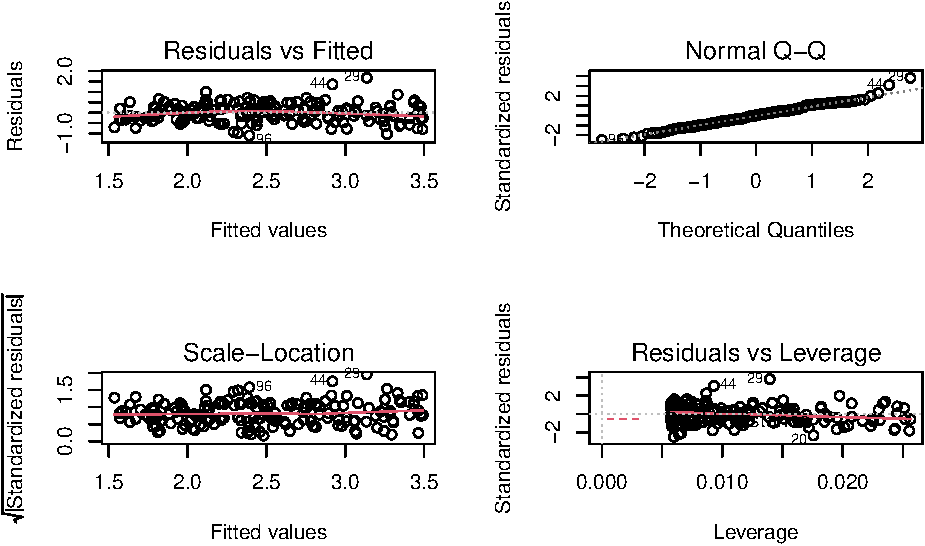
\includegraphics[width=0.7\linewidth]{10-regression_files/figure-latex/unnamed-chunk-2-1} \end{center}

\begin{enumerate}
\def\labelenumi{\arabic{enumi}.}
\setcounter{enumi}{3}
\tightlist
\item
  Describe the features of the plot you created in Question 3.
\end{enumerate}

\vspace{1in}

If you indicated there are potential outliers, which points are they?

\hypertarget{conditions-for-the-least-squares-line}{%
\subsection{Conditions for the least squares line}\label{conditions-for-the-least-squares-line}}

When performing inference on a least squares line, the follow conditions are generally required

\begin{itemize}
\tightlist
\item
  Linearity: the data should follow a linear trend
\item
  Nearly normal residuals: residuals must be nearly normal
\item
  Constant variability: the variability of points around the least squares line remains roughly constant
\item
  Independent observations: individual data points must be independent
\end{itemize}

The scatterplot and the residual plot will be used to assess the conditions for approximating the data with the T-distribution

\begin{center}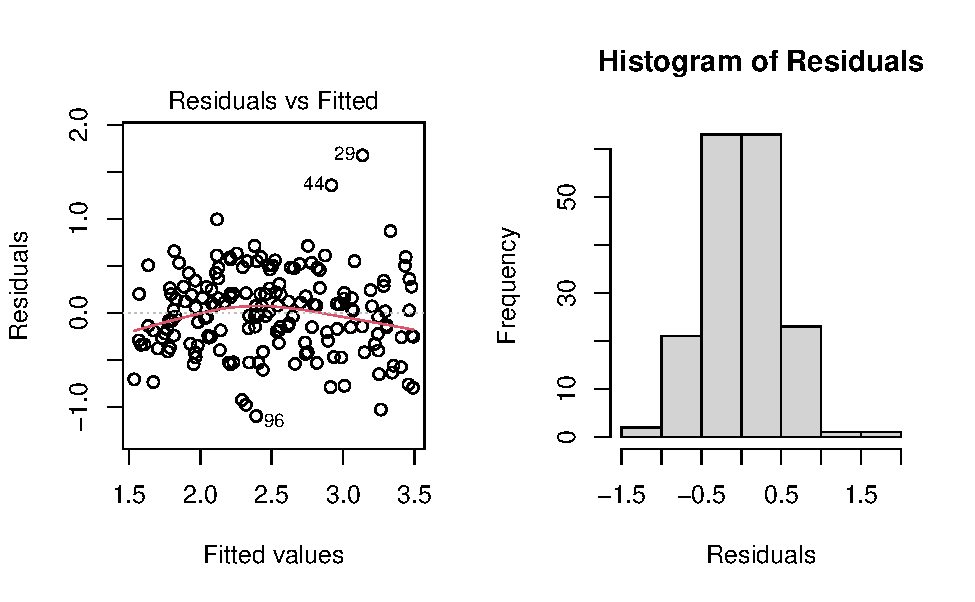
\includegraphics[width=0.7\linewidth]{10-regression_files/figure-latex/unnamed-chunk-3-1} \end{center}

\begin{enumerate}
\def\labelenumi{\arabic{enumi}.}
\setcounter{enumi}{4}
\tightlist
\item
  Are the conditions met
\end{enumerate}

\vspace{1in}

\hypertarget{ask-a-reseach-question}{%
\subsection{Ask a reseach question}\label{ask-a-reseach-question}}

\begin{enumerate}
\def\labelenumi{\arabic{enumi}.}
\setcounter{enumi}{5}
\tightlist
\item
  Write out the null hypothesis in words.
\end{enumerate}

\vspace{1in}

\begin{enumerate}
\def\labelenumi{\arabic{enumi}.}
\setcounter{enumi}{6}
\tightlist
\item
  Using the research question, write the alternative hypothesis in notation.
\end{enumerate}

\vspace{0.5in}

\hypertarget{summarize-and-visualize-the-data}{%
\subsection{Summarize and visualize the data}\label{summarize-and-visualize-the-data}}

Enter the variable names into the linear model function to get the linear model output.

\begin{verbatim}
#>              Estimate  Std. Error  t value     Pr(>|t|)
#> (Intercept) 1.1070563 0.093326769 11.86215 4.237698e-24
#> age         0.1404378 0.008796699 15.96483 8.777516e-36
\end{verbatim}

\begin{enumerate}
\def\labelenumi{\arabic{enumi}.}
\setcounter{enumi}{7}
\tightlist
\item
  Using the output above, write the equation of the regression line.
\end{enumerate}

\vspace{1in}

\begin{enumerate}
\def\labelenumi{\arabic{enumi}.}
\setcounter{enumi}{8}
\tightlist
\item
  Interpret the slope in context of the problem.
\end{enumerate}

\vspace{1in}

\begin{enumerate}
\def\labelenumi{\arabic{enumi}.}
\setcounter{enumi}{9}
\tightlist
\item
  Using your estimated line of best fit, predict the per peg speed for a participant who was 9.18 years old. Show all work.
\end{enumerate}

\vspace{1in}

\begin{enumerate}
\def\labelenumi{\arabic{enumi}.}
\setcounter{enumi}{10}
\tightlist
\item
  Calculate the residual associated with the observation (9.18, 2.95), using your estimated regression line from question 8.
\end{enumerate}

\vspace{1in}

\hypertarget{use-statistical-inferential-methods-to-draw-inferences-from-the-data}{%
\subsection{Use statistical inferential methods to draw inferences from the data}\label{use-statistical-inferential-methods-to-draw-inferences-from-the-data}}

To find the value of the test statistic to test the slope we will use,

\(T = \frac{\mbox{slope estimate}}{SE} = T = \frac{b_1}{SE(b_1)}\)

We will use the linear model output above to get the estimate for slope and standard error.

\begin{enumerate}
\def\labelenumi{\arabic{enumi}.}
\setcounter{enumi}{11}
\tightlist
\item
  Calculate the test statistic for slope.
\end{enumerate}

\vspace{1in}

\begin{enumerate}
\def\labelenumi{\arabic{enumi}.}
\setcounter{enumi}{12}
\tightlist
\item
  What value does the value calculated in question 12 match in the linear model output?
\end{enumerate}

\vspace{0.5in}

\begin{enumerate}
\def\labelenumi{\arabic{enumi}.}
\setcounter{enumi}{13}
\tightlist
\item
  Interpret the test statistic in context of the problem.
\end{enumerate}

\vspace{1in}

\begin{enumerate}
\def\labelenumi{\arabic{enumi}.}
\setcounter{enumi}{14}
\tightlist
\item
  Using the linear model output, report the p-value for the test of significance.
\end{enumerate}

\vspace{0.5in}

\begin{enumerate}
\def\labelenumi{\arabic{enumi}.}
\setcounter{enumi}{15}
\tightlist
\item
  Based on the p-value, how much evidence is there against the null hypothesis?
\end{enumerate}

\vspace{0.5in}

Recall that a confidence interval is calculated by adding and subtracting the margin of error to the point estimate.

\(\mbox{point estimate}\pm t^*SE(estimate)\)
\(b_1 \pm t^* SE(b_1)\)

The \(t^*\) multiplier comes from the t-distribution with \(n-2\) df.

\begin{verbatim}
#> [1] 1.973852
\end{verbatim}

\begin{enumerate}
\def\labelenumi{\arabic{enumi}.}
\setcounter{enumi}{16}
\item
  Calculate the 95\% confidence interval for the true slope.
  \vspace{1in}
\item
  Calculate the coefficient of determination for a linear model that describes the relationship between \texttt{age} and \texttt{speed}. Use proper notation.
\end{enumerate}

\vspace{1in}

\begin{enumerate}
\def\labelenumi{\arabic{enumi}.}
\setcounter{enumi}{18}
\tightlist
\item
  Interpret this value in the context of the study.
\end{enumerate}

\vspace{1in}

\hypertarget{communicate-the-results-and-answer-the-research-question}{%
\subsection{Communicate the results and answer the research question}\label{communicate-the-results-and-answer-the-research-question}}

\begin{enumerate}
\def\labelenumi{\arabic{enumi}.}
\setcounter{enumi}{19}
\tightlist
\item
  Based on the p-value, write a conclusion in context of the problem.
\end{enumerate}

\vspace{1in}

\begin{enumerate}
\def\labelenumi{\arabic{enumi}.}
\setcounter{enumi}{20}
\tightlist
\item
  Interpret the 95\% confidence interval in context of the problem.
\end{enumerate}

\vspace{1in}

\begin{enumerate}
\def\labelenumi{\arabic{enumi}.}
\setcounter{enumi}{21}
\tightlist
\item
  Summarize the results of the study in a written paragraph. Be sure to include.
\end{enumerate}

\begin{itemize}
\item
  Summary statistic
\item
  Test statistic and interpretation
\item
  P-value and interpretation
\item
  Confidence interval and interpretation
\item
  Conclusion in context
\item
  Scope of inference
\end{itemize}

\hypertarget{revisit-and-look-forward}{%
\subsection{Revisit and look forward}\label{revisit-and-look-forward}}

\begin{enumerate}
\def\labelenumi{\arabic{enumi}.}
\setcounter{enumi}{22}
\tightlist
\item
  Is there an effect due to gender on this linear relationship? Explain your answer using the scatterplot.
\end{enumerate}

\begin{center}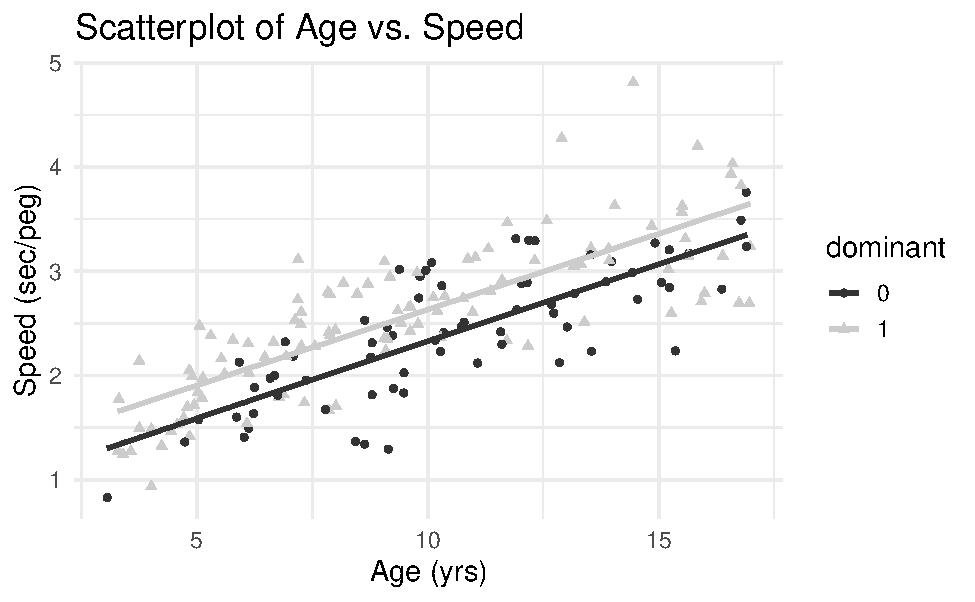
\includegraphics[width=0.7\linewidth]{10-regression_files/figure-latex/unnamed-chunk-6-1} \end{center}

\hypertarget{additional-notes}{%
\section{Additional notes}\label{additional-notes}}

Use this space to summarize your thoughts and take additional notes on today's activity.

\end{document}
